% Chapter 12 -- The Low-Risk Anomaly
% Requires: amsmath, amssymb, booktabs, array, tabularx, graphicx, tcolorbox (breakable, skins), hyperref or url.
% Defines the callout box only if the preamble has not.
\providecolor{fenavy}{HTML}{1B2A6B}
\providecolor{feshade}{HTML}{F3F5FA}
\makeatletter
\@ifundefined{callout}{%
  \newtcolorbox{callout}{breakable, enhanced,
    colback=white, colframe=gray!70, boxrule=0.5pt, arc=1mm,
    borderline west={2.5pt}{0pt}{gray!70},
    left=8pt, right=8pt, top=4pt, bottom=4pt}%
}{}
\makeatother

\chapter{The Low-Risk Anomaly}
\label{ch:12}

The capital asset pricing model makes one central prediction: assets that move more with the market should earn more. Double the beta, double the expected excess return. It is the first model most finance students learn and the one most practitioners still use to set hurdle rates.

The prediction was also among the first to be tested, and it failed early. In the 1970s Black, Jensen and Scholes found that the relation between beta and average return was positive but far flatter than the CAPM implied. Since then the finding has been extended in two directions. Stocks with low \emph{volatility}, not just low beta, have earned more than their risk suggests. And the pattern appears in other countries and asset classes. It is now usually called the \textbf{low-risk anomaly}.

This chapter asks whether the low-risk anomaly is a real and usable premium or something weaker: a tilt toward small or profitable firms, a disguised bet on interest rates, or a pattern that faded once low-volatility funds became popular after 2010.

By the end of the chapter you will be able to:

\begin{itemize}
  \item estimate a beta, split total risk into systematic and idiosyncratic parts, and compute a CAPM alpha;
  \item draw the security market line and explain how leverage constraints flatten it;
  \item build a beta-neutral betting-against-beta portfolio and explain why a naive low-minus-high portfolio can lose money despite a positive alpha;
  \item state the weak and strong forms of the low-risk claim and summarize the evidence for each;
  \item compare the explanations: leverage constraints, lottery preferences, benchmarking, and missing risk factors;
  \item judge whether a minimum-volatility or BAB fund delivers what its backtest promises.
\end{itemize}

\section{Foundations: beta, the CAPM and the security market line}
\label{sec:12-foundations}

\textbf{Beta} measures how much an asset moves with the market:
\begin{equation}
  \beta_i = \frac{\mathrm{Cov}(R_i, R_m)}{\mathrm{Var}(R_m)}
  \label{eq:12-beta}
\end{equation}
In practice it is the slope of a regression of the asset's excess return on the market's excess return. The market itself has a beta of 1. A stock with a beta of 1.5 tends to rise 1.5\% when the market rises 1\%, and to fall 1.5\% when it falls 1\%.

\textbf{Total risk} splits into two parts. \textbf{Systematic risk} is $\beta_i^2\,\mathrm{Var}(R_m)$. \textbf{Idiosyncratic risk} is the variance of the regression residual, which diversification removes. Two stocks can have the same volatility but very different betas.

The \textbf{CAPM} (Sharpe 1964, Lintner 1965) says that only systematic risk is priced:
\begin{equation}
  E[R_i] - R_f = \beta_i \left(E[R_m] - R_f\right)
  \label{eq:12-capm}
\end{equation}
Plotting expected return against beta gives the \textbf{security market line (SML)}. It is a straight line through the risk-free rate at $\beta = 0$ and the market at $\beta = 1$, so its slope equals the market premium. Idiosyncratic risk earns nothing, because investors can diversify it away for free.

\textbf{Alpha} (Jensen's alpha) is the intercept $\alpha_i$ in the regression
\begin{equation}
  R_i - R_f = \alpha_i + \beta_i (R_m - R_f) + \varepsilon_i
  \label{eq:12-alpha}
\end{equation}
It measures average return beyond what beta explains. Under the CAPM every alpha is zero. A \textbf{multifactor alpha} adds other factors to the regression, such as size, value and momentum (Chapter 8).

The CAPM assumes that investors can borrow and lend freely at the risk-free rate. An investor who wants more risk than the market then borrows and buys the market, or any efficient portfolio. Many investors cannot do this. Mutual funds and pension plans face limits on \textbf{leverage}, borrowing to hold more than their capital. Individuals face \textbf{margin} requirements and pay more than the risk-free rate to borrow. Black (1972) showed that without riskless borrowing the SML is still straight but flatter: it starts at the return on a \textbf{zero-beta portfolio}, a portfolio uncorrelated with the market, which lies above the risk-free rate.

\textbf{Worked example.} The risk-free rate is 3\% and the market premium is 6\% (Figure~\ref{fig:12-sml}).

\begin{itemize}
  \item Stock A has a beta of 0.6 and has averaged 9\%. The CAPM predicts $3\% + 0.6 \times 6\% = 6.6\%$, so A's alpha is $+2.4\%$.
  \item Stock B has a beta of 1.5 and has averaged 10\%. The CAPM predicts $3\% + 1.5 \times 6\% = 12\%$, so B's alpha is $-2\%$.
  \item An investor who can borrow at 3\% can lever A to a beta of 1. She holds $1/0.6 = 1.67$ dollars of A for each dollar of capital and borrows the remaining 0.67 dollars. Her expected return is $3\% + 1.67 \times (9\% - 3\%) = 13\%$, compared with 9\% for the market at the same beta. Even at a borrowing rate of 5\%, she earns $1.67 \times 9\% - 0.67 \times 5\% \approx 11.7\%$.
  \item An investor who cannot borrow and wants a beta above 1 must buy B instead. If many investors are in that position, they bid up high-beta stocks such as B and push down their future returns. That is the core of the leverage-constraint explanation in Section~\ref{sec:12-explanations}.
\end{itemize}

\begin{figure}[htbp]
\centering
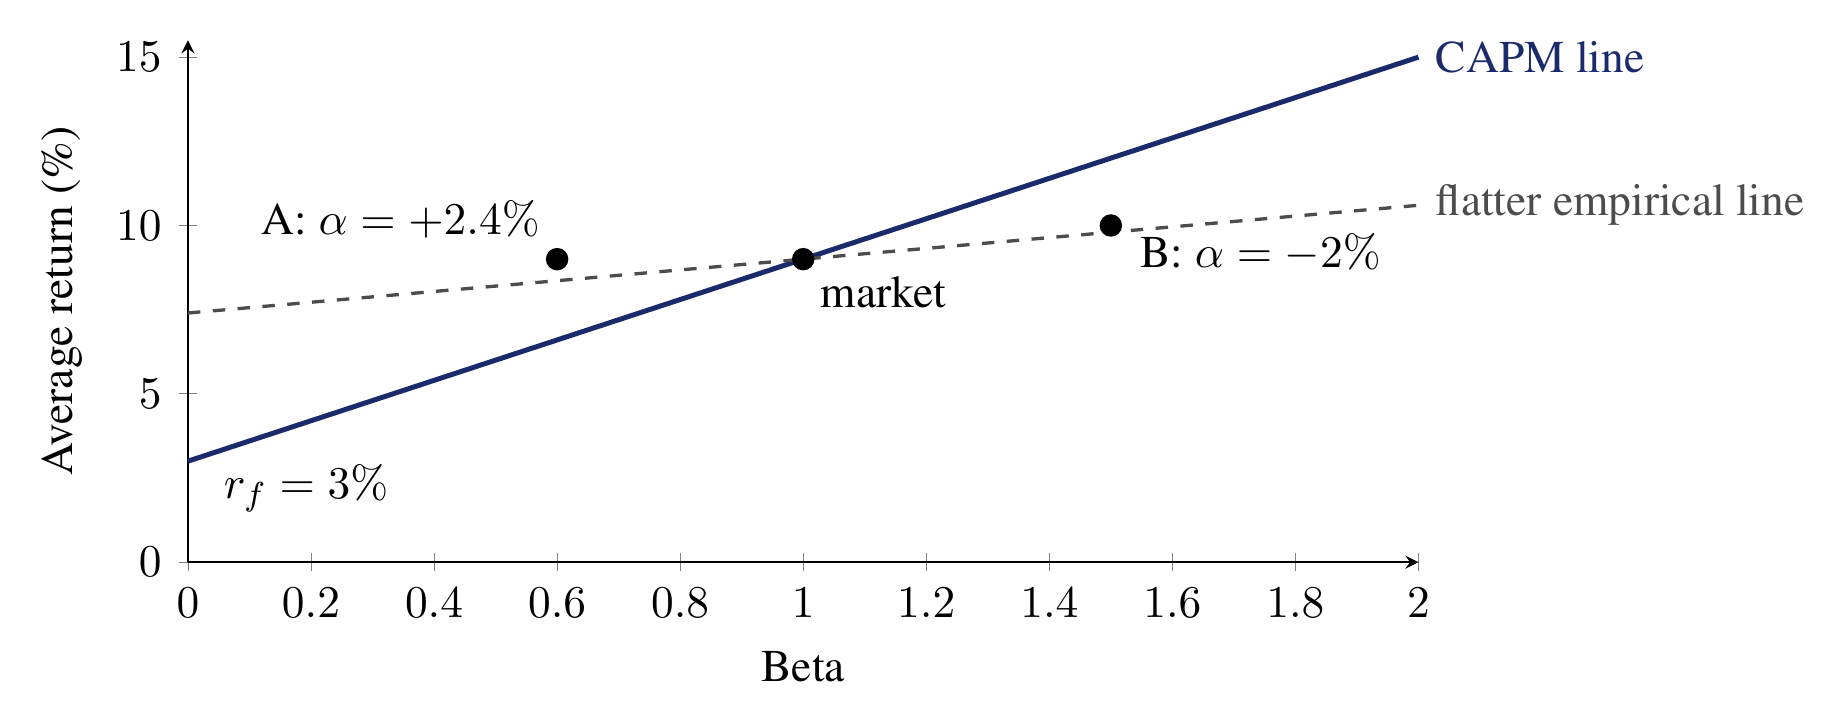
\includegraphics[width=0.85\linewidth]{images/fig12-1-sml.png}
\caption{The security market line in the worked example. The CAPM line runs from the risk-free rate of 3\% through the market at a beta of 1. Stock A lies above it (positive alpha) and stock B below it (negative alpha), so the line through A and B is flatter than the CAPM predicts.}
\label{fig:12-sml}
\end{figure}

\textbf{Further reading.} Bodie, Kane and Marcus, \emph{Investments} (the CAPM, the index model and beta estimation, and empirical tests of the CAPM); Cochrane, \emph{Asset Pricing} (beta pricing models and their tests); Campbell, Lo and MacKinlay, \emph{The Econometrics of Financial Markets} (tests of the CAPM); Ang, \emph{Asset Management} (low-risk anomalies from an investor's viewpoint).

\section{How it works}
\label{sec:12-how}

There are three ways to sort stocks on risk, and the literature uses all three.

\begin{itemize}
  \item \textbf{Beta.} Estimate each stock's beta from past returns, typically 36 to 60 months of monthly data or a year of daily data. Sort into portfolios. This tests the CAPM directly.
  \item \textbf{Total volatility.} Sort on the standard deviation of past daily returns, often over one to three months. This needs no market model, and it is how most low-volatility funds work.
  \item \textbf{Idiosyncratic volatility.} Sort on the volatility of residuals from a factor model, usually the Fama--French three-factor model. Under the CAPM this risk should not be priced at all, so a negative relation is especially puzzling.
\end{itemize}

The three measures are strongly correlated. High-beta stocks tend to be volatile, and volatile stocks tend to have high idiosyncratic risk. Separating them is one of the open problems in this chapter.

A flat SML shows up in two ways. The first is \emph{alphas}: low-risk portfolios have positive CAPM alphas and high-risk portfolios negative ones. The second is a \emph{long-short portfolio}. The naive version, long low-risk stocks and short high-risk stocks, has a strongly negative beta. It loses money in rising markets even if the SML is flat, and its average return can be negative while its alpha is positive. \textbf{Betting against beta (BAB)} fixes this. It levers the low-beta leg up to a beta of 1 and scales the high-beta leg down to a beta of 1, so the portfolio is \textbf{beta-neutral}, with no net exposure to the market (Figure~\ref{fig:12-bab}):
\begin{equation}
  r_{\mathrm{BAB}} = \frac{r_L - r_f}{\beta_L} - \frac{r_H - r_f}{\beta_H}
  \label{eq:12-bab}
\end{equation}
If the SML is flat, this portfolio earns a positive return with no market exposure. The betas must be \textbf{ex ante}, estimated from data available when the portfolio is formed. Otherwise the construction looks ahead (Section~\ref{sec:02-lookahead}).

\begin{figure}[htbp]
\centering
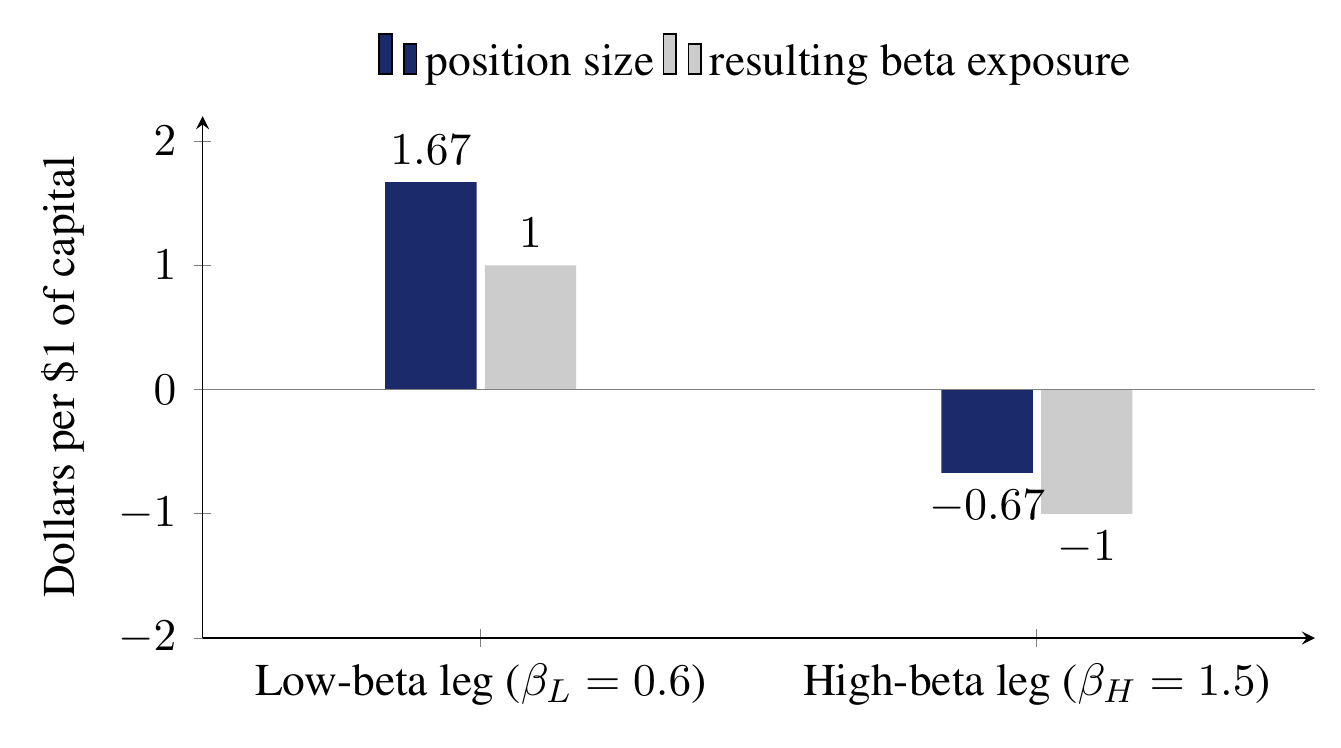
\includegraphics[width=0.85\linewidth]{images/fig12-2-bab.png}
\caption{Building a BAB portfolio from the worked example. Per dollar of capital, it holds \$1.67 of the low-beta stock ($\beta_L = 0.6$) and shorts \$0.67 of the high-beta stock ($\beta_H = 1.5$). Each leg then carries a beta exposure of 1, in opposite directions, so the portfolio's beta is zero.}
\label{fig:12-bab}
\end{figure}

The explanations divide into those that treat the anomaly as \textbf{mispricing} and those that treat it as \textbf{compensation for a risk the CAPM misses}. Section~\ref{sec:12-explanations} sets them out. They matter because they predict different things about when the anomaly should be strongest, and about whether it should survive its own popularity.

\section{The claim}
\label{sec:12-claim}

\begin{callout}
\textbf{Claim.} Low-beta and low-volatility stocks earn higher risk-adjusted returns than the CAPM predicts. The security market line is flatter than the market premium, and a beta-neutral portfolio that is long low-risk stocks and short high-risk stocks earns a positive alpha.
\end{callout}

To test it we need to specify four things.

\begin{itemize}
  \item \textbf{The strong form.} The SML is not just flat but \emph{inverted}: low-risk stocks earn higher raw returns, not just higher risk-adjusted returns. Some studies of volatility sorts find this. Most studies of beta sorts find a flat or weakly positive relation instead.
  \item \textbf{The weak form.} The SML is positive but flatter than the CAPM predicts, so low-beta stocks have positive alphas. This is what Black, Jensen and Scholes found, and it is the claim tested here.
  \item \textbf{Risk adjustment.} A CAPM alpha is the natural first test. The claim is more interesting if the alpha survives the size, value and momentum factors, and more interesting still if it survives profitability and interest-rate exposure.
  \item \textbf{What would count against it.} The claim weakens if the alpha is concentrated in micro-caps, if it disappears after controlling for other known factors, or if it has faded since the strategy became popular. It fails if a beta-neutral, tradable version earns nothing after costs.
\end{itemize}

\section{The original evidence}
\label{sec:12-evidence}

\textbf{A flat line from the start.} Black, Jensen and Scholes (1972) sorted NYSE stocks from 1931 to 1965 into ten portfolios by past beta, so that estimation error in individual betas would average out. Average returns rose with beta, but much less than the CAPM predicted. Low-beta portfolios had positive alphas and high-beta portfolios negative ones. Fama and MacBeth (1973) confirmed a positive but modest slope. Haugen and Heins (1975) reported that low-volatility portfolios had matched or beaten high-volatility ones, and Fama and French (1992) found almost no relation between beta and average return from 1963 to 1990 once size was controlled for.

\textbf{Idiosyncratic volatility.} Ang, Hodrick, Xing and Zhang (2006) sorted U.S. stocks on idiosyncratic volatility measured over the previous month. The highest-volatility quintile earned 1.06\% a month less than the lowest, and its Fama--French alpha was 1.31\% a month lower. The result was a strong form of the anomaly: an inverted relation between this risk and raw returns. Their 2009 paper found the same pattern in 23 developed markets.

\textbf{From anomaly to strategy.} Baker, Bradley and Wurgler (2011) documented the low-risk anomaly for investors and argued that benchmarking prevents institutions from exploiting it. Frazzini and Pedersen (2014) built the BAB factor described in Section~\ref{sec:12-how} from individual stocks, using rank weights and shrunk betas. In U.S. stocks from 1926 to 2012 it had a Sharpe ratio of 0.78. It earned significant alphas after size, value, momentum and liquidity controls, in 19 international equity markets, and in Treasury bonds, corporate bonds and futures. They also found that BAB returns were lower when funding constraints were tight, which their leverage-constraint theory predicts.

By 2014 the low-risk anomaly looked like one of the best-documented patterns in finance. Low-volatility index funds launched in the United States around 2011 and grew quickly.

\section{Explanations}
\label{sec:12-explanations}

\textbf{Leverage constraints.} Black (1972) and Frazzini and Pedersen (2014) argue that investors who want high expected returns but cannot borrow overweight high-beta stocks instead of levering the market. That bids up high-beta stocks and flattens the SML. The theory predicts that constrained investors, such as mutual funds and individuals, hold high-beta portfolios, and that BAB does worse when funding tightens. Both predictions have empirical support.

\textbf{Lottery preferences.} Some investors like stocks with a small chance of a very large gain, as with a lottery ticket, and overpay for them. Barberis and Huang (2008) derive this from probability weighting in prospect theory. Bali, Cakici and Whitelaw (2011) found that stocks with the largest daily returns over the past month subsequently underperform, and that this absorbs much of the idiosyncratic volatility effect. Lottery demand explains volatility sorts more naturally than beta sorts.

\textbf{Benchmarking.} Most institutional managers are judged against a capitalization-weighted index. For them, a low-beta stock with positive alpha is not attractive: it adds \textbf{tracking error}, the volatility of the return difference from the benchmark, and lags in rising markets. Baker, Bradley and Wurgler (2011) argue that this keeps institutions from correcting the mispricing. Part D of the lab measures how large that tracking error is.

\textbf{Overpricing that is hard to short.} Liu, Stambaugh and Yuan (2018) found that the beta anomaly comes from beta's correlation with idiosyncratic volatility, and that it is concentrated among overpriced stocks, where short-selling is costly.

\textbf{Missing risk factors.} Other explanations treat the alpha as compensation for risks the CAPM omits.

\begin{itemize}
  \item \emph{Profitability and investment.} Low-risk stocks tend to be large, profitable and conservative in investment. Fama and French (2016) found that their five-factor model, which adds profitability and investment factors, explains much of the low-beta and low-volatility alphas.
  \item \emph{Interest rates.} Low-volatility stocks, such as utilities and consumer staples, behave partly like bonds. Driessen, Kuiper, Nazliben and Beilo (2019) found that low-volatility portfolios lose value when rates rise and that an interest-rate premium explains part, but not all, of the anomaly. Over 1981--2020 bond yields fell almost continuously, which would have flattered any bond-like equity strategy.
  \item \emph{Conditional betas.} Cederburg and O'Doherty (2016) found that betas vary over time in ways that bias unconditional alphas, and that modelling time-varying betas largely eliminates the alpha gap between low- and high-beta stocks.
\end{itemize}

The explanations are not mutually exclusive. Asness, Frazzini, Gormsen and Pedersen (2020) split BAB into a bet against correlation, which they link to leverage constraints, and a bet against volatility, which they link to lottery demand, and report that both earn returns.

\section{Replication lab: the security market line since 1963}
\label{sec:12-lab}

\begin{callout}
\textbf{Lab 12 at a glance.} \emph{Claim on trial:} low-risk stocks earn more than the CAPM predicts. \emph{Data:} ten portfolios formed on market beta, on total variance and on residual variance, each value- and equal-weighted, from July 1963, from the Kenneth French library; the Fama--French and momentum factors; the 10-year Treasury yield from FRED; optionally, AQR's published BAB factor for comparison. All are free. \emph{Code:} runs as a script (\texttt{python lab12.py}) or as a notebook with a prediction prompt before each step.
\end{callout}

\textbf{Part A, the SML.} For each set of decile portfolios, the lab estimates average excess return, realized beta, CAPM alpha and four-factor alpha, and the slope of average return on beta across the deciles. Figure 12.3 plots the deciles against the CAPM line, which runs from the origin through the market.

\textbf{Part B, long-short portfolios.} Two constructions for each sort:

\begin{center}
\small
\begin{tabularx}{0.9\linewidth}{@{}>{\raggedright\arraybackslash}p{0.19\linewidth}>{\raggedright\arraybackslash}X>{\raggedright\arraybackslash}X>{\raggedright\arraybackslash}p{0.17\linewidth}@{}}
\toprule
Construction & Long & Short & Beta \\
\midrule
Low minus high & Three lowest-risk deciles & Three highest-risk deciles & Strongly negative \\
BAB-style & Low leg $\times\, 1/\beta_L$ & High leg $\times\, 1/\beta_H$ & About zero \\
\bottomrule
\end{tabularx}
\end{center}

The betas are estimated from the previous 60 months of each leg's returns, so the portfolio uses only information available at the time. Figure 12.4 plots cumulative returns.

This is a simpler construction than Frazzini and Pedersen's. They use individual stocks with rank weights. The lab uses published portfolios, which anyone can reproduce in minutes. Expect it to show the same pattern with smaller numbers, partly because it does not tilt toward small stocks. Comparing it with AQR's factor (optional) shows how much the construction matters.

\textbf{Part C, stress tests.} Equal versus value weights, three subperiods (1963--1990, 1991--2009, 2010 onward), interest-rate exposure, calendar-year returns in 2008, 2020 and 2022, and rolling ten-year alphas (Figures 12.5 and 12.6).

\textbf{Part D, the investor's view.} The lowest-volatility and lowest-beta quintiles against the market: Sharpe ratio, alpha, drawdown, tracking error and the share of years in which they trailed the market (Figure 12.7).

\textbf{What the simulated run shows.} On simulated data built with a flat SML, the lab recovers what it should. The slope across beta deciles is far below the market premium. The BAB-style portfolios have betas near zero and positive alphas. The low-minus-high portfolio sorted on beta loses money on average despite its positive alpha, which illustrates why the construction matters. These results confirm that the code works. They say nothing about real markets. Run the lab on the real data to reach your own verdict.

\section{Stress tests}
\label{sec:12-stress}

\textbf{Micro-caps and weighting.} Novy-Marx and Velikov (2022) found that AQR's BAB factor, through its rank weighting and leverage, commits on average about \$1.05 of each dollar to the smallest 1\% of stocks by market capitalization. Those stocks are expensive to trade (Chapter 6). After costs BAB still earned positive returns, but they attribute part of them to exposure to profitability and investment. The lab's equal- versus value-weighted comparison is a coarse version of this test. If the effect is much stronger in equal-weighted portfolios, small stocks are doing much of the work (Section~\ref{sec:02-microcaps}).

\textbf{Other factors.} Fama and French (2016) found that profitability and investment factors absorb much of the low-risk alphas. The lab uses four factors, so its alphas probably overstate what remains. Exercise 6 adds the five-factor model.

\textbf{Interest rates.} If low-risk stocks are partly bonds, their alpha includes a bond premium earned during four decades of falling yields. The lab regresses the long-short returns and the low-risk leg on the market and on monthly changes in the 10-year yield. A negative coefficient means the strategy loses when yields rise. 2022 is the natural out-of-sample test: yields rose sharply, and stocks and bonds fell together.

\textbf{Crowding.} Low-volatility funds grew rapidly after 2011. If the anomaly reflected mispricing, the inflows should have raised the prices of low-risk stocks, boosting returns at first and lowering them afterward. The lab's 2010-onward subperiod and the rolling alphas in Figure 12.5 show whether the premium has shrunk.

\textbf{Drawdowns.} Low-risk portfolios are meant to protect in crashes. Check 2008 and March 2020. A beta-neutral BAB portfolio is a different matter. It is long levered low-beta stocks and short high-beta stocks, and it can lose heavily when high-beta stocks rebound sharply, as in 2009 and in the 2020 recovery.

\textbf{Estimation error in beta.} Sorting on noisy past betas means the low-beta portfolio contains stocks whose true betas are higher than estimated, and the reverse. This biases the SML toward flatness even if the CAPM holds. Black, Jensen and Scholes used portfolios to reduce the problem, and the French portfolios do the same. Novy-Marx and Velikov (2022) also showed that Frazzini and Pedersen's beta estimator, which combines correlations and volatilities measured over different windows, introduces its own biases.

\section{Verdict}
\label{sec:12-verdict}

\begin{callout}
\textbf{Verdict: weakens} (as of October 2026). The weak form of the claim, that the security market line is flatter than the CAPM predicts, is one of the most robust findings in empirical finance. The strong form, that low-risk stocks earn a distinct premium that a beta-neutral portfolio can harvest, is weaker. Its size depends heavily on construction and on micro-caps, much of it overlaps with profitability, investment and interest-rate exposure, and the evidence that it is a separate premium is weaker than it looked in 2014.
\end{callout}

What survives:

\begin{itemize}
  \item \textbf{The flat SML.} Since Black, Jensen and Scholes, beta sorts have shown a relation between beta and average return that is much flatter than the market premium, in the United States and abroad. A CAPM hurdle rate overstates the expected return of high-beta assets relative to low-beta ones.
  \item \textbf{Low risk without lower returns.} Low-volatility portfolios have delivered returns close to the market's with substantially less volatility, so their Sharpe ratios have been higher. For an unconstrained investor that is useful.
\end{itemize}

What weakens it:

\begin{itemize}
  \item \textbf{Construction.} Rank-weighted, stock-level BAB factors put much of their capital in the smallest stocks (Novy-Marx and Velikov 2022). Portfolio-based versions, like the lab's, earn less.
  \item \textbf{Overlap with other factors.} Profitability and investment factors explain much of the alpha (Fama and French 2016). Time-varying betas explain much of the rest (Cederburg and O'Doherty 2016).
  \item \textbf{Interest rates.} Low-risk stocks behave partly like bonds, and the sample is dominated by four decades of falling yields.
  \item \textbf{Crowding.} Inflows into low-volatility funds after 2011 are likely to have raised the prices of low-risk stocks, which would make past returns a poor guide to future ones.
\end{itemize}

The verdict would move to \emph{survives} if a beta-neutral, value-weighted version continued to earn a significant alpha against the five-factor model and interest-rate exposure out of sample. It would move to \emph{fails} if the post-2010 alphas proved to be inflow effects that reversed.

\section{What investors can use}
\label{sec:12-investors}

\textbf{Minimum-volatility funds} are the most common way investors access the low-risk anomaly. They hold a portfolio of stocks chosen or optimized for low volatility, usually long-only and without leverage. Three things are worth knowing before buying one.

\begin{itemize}
  \item \textbf{They are low-beta, not market-neutral.} With a beta around 0.7 to 0.8, a minimum-volatility fund will usually trail the market in strong bull markets and beat it in crashes. The case for holding one rests on a better ratio of return to risk, not higher returns.
  \item \textbf{Tracking error is large.} For an investor measured against the market, the fund can lag for years at a time. Part D of the lab shows how often. Investors who cannot tolerate that, including most institutions, are the reason Baker, Bradley and Wurgler think the anomaly persists. Investors who abandon the strategy after a few bad years lose most of its benefit.
  \item \textbf{Hidden exposures.} These funds tend to overweight utilities, consumer staples and real estate, which are sensitive to interest rates. Their valuations can rise with the strategy's popularity. An investor should check the sector weights, the valuation relative to the market, and how the fund behaved when yields rose.
\end{itemize}

\textbf{BAB-style funds}, long levered low-beta stocks and short high-beta stocks, are a different product. They are market-neutral, carry the micro-cap and leverage issues discussed above, and can suffer sharp losses when high-beta stocks rebound.

\textbf{Questions to ask a manager offering a low-volatility or defensive equity strategy:}

\begin{itemize}
  \item Is the portfolio sorted on beta, on volatility or on an optimizer's estimate of risk? How much tracking error should I expect against the market?
  \item What are the strategy's sector weights and interest-rate sensitivity? How did it perform in 2022?
  \item Does the backtest include micro-caps? What is its alpha against the five-factor model?
  \item How have valuations of low-volatility stocks changed since the strategy became popular?
\end{itemize}

\begin{callout}
\textbf{What Failed: the CAPM as a hurdle rate.} The CAPM's empirical problems have been known since the early 1970s, yet it remains the standard way to set the cost of equity. In a survey of 392 U.S. CFOs, Graham and Harvey (2001) found that 73.5\% of respondents always or almost always used it. A flat SML means that the CAPM overstates the cost of capital for high-beta projects and understates it for low-beta ones. Firms that rely on it may reject good low-beta projects and accept poor high-beta ones.

The lesson is not that the CAPM is useless. Beta is a good measure of exposure to the market, and that is what risk management needs. The failure is treating a model of \emph{risk} as a reliable model of \emph{expected return} when the evidence has long said otherwise.
\end{callout}

\section{Open questions}
\label{sec:12-open}

\begin{itemize}
  \item \textbf{How much is interest-rate exposure?} Low-risk stocks lose when yields rise. Is the remaining alpha, after controlling for rates, large enough to matter, and how did the strategy hold up in the rising-rate environment after 2021?
  \item \textbf{Which risk measure is priced?} Beta, total volatility and idiosyncratic volatility are highly correlated. Leverage-constraint theories favor beta; lottery theories favor volatility. Which survives when the others are controlled for?
  \item \textbf{Has crowding ended the premium?} Inflows into low-volatility funds should have produced a temporary windfall followed by lower returns. Is the post-2010 evidence consistent with that?
  \item \textbf{Does it hold for large stocks after costs?} A value-weighted, beta-neutral portfolio of liquid stocks is the version that matters for most investors. How large is its alpha against the five-factor model?
\end{itemize}

\section*{Exercises}
\addcontentsline{toc}{section}{Exercises}

\subsection*{Conceptual (all readers)}

\begin{enumerate}
  \item The risk-free rate is 4\% and the market premium 5\%. Stock X has a beta of 0.7 and an expected return of 9\%; stock Y has a beta of 1.4 and an expected return of 10\%. (a) Compute each alpha. (b) Build a beta-neutral BAB portfolio from X and Y. What is its expected return? (c) How does your answer change if borrowing costs 6\%?
  \item Explain why estimation error in individual betas flattens the estimated SML, and why sorting into portfolios helps.
\end{enumerate}

\subsection*{Lab extensions (technical readers)}

\begin{enumerate}
  \setcounter{enumi}{2}
  \item Part A: compare the SML slope for beta-sorted and volatility-sorted deciles, value- and equal-weighted. Which shows the flattest relation?
  \item Part B: explain why the low-minus-high portfolio sorted on beta can have a negative average return and a positive alpha at the same time.
  \item Part B: download AQR's BAB factor and compare it with the lab's BAB-style portfolio. What is their correlation? Which has the higher alpha, and why might that be?
  \item Part C: add the five-factor model (download the Fama--French 5-factor file). How much of each low-risk alpha remains?
  \item Part C: using the interest-rate regression, estimate the ``duration'' of the low-volatility leg. How much of its 2022 return does the rise in yields explain?
  \item Part D: find the longest period in which the lowest-volatility quintile trailed the market. Would you have kept a manager through it?
  \item A pension fund asks whether to move 20\% of its equities into a minimum-volatility fund. Write a one-page memo that uses the evidence in this chapter, including the case against.
\end{enumerate}

\section*{References}
\addcontentsline{toc}{section}{References}

\begin{itemize}
  \item Ang, A., Hodrick, R. J., Xing, Y. and Zhang, X. (2006). The Cross-Section of Volatility and Expected Returns. \emph{Journal of Finance} 61(1): 259--299.
  \item Ang, A., Hodrick, R. J., Xing, Y. and Zhang, X. (2009). High Idiosyncratic Volatility and Low Returns: International and Further U.S. Evidence. \emph{Journal of Financial Economics} 91(1): 1--23.
  \item Asness, C., Frazzini, A., Gormsen, N. J. and Pedersen, L. H. (2020). Betting against Correlation: Testing Theories of the Low-Risk Effect. \emph{Journal of Financial Economics} 135(3): 629--652.
  \item Baker, M., Bradley, B. and Wurgler, J. (2011). Benchmarks as Limits to Arbitrage: Understanding the Low-Volatility Anomaly. \emph{Financial Analysts Journal} 67(1): 40--54.
  \item Bali, T. G., Cakici, N. and Whitelaw, R. F. (2011). Maxing Out: Stocks as Lotteries and the Cross-Section of Expected Returns. \emph{Journal of Financial Economics} 99(2): 427--446.
  \item Barberis, N. and Huang, M. (2008). Stocks as Lotteries: The Implications of Probability Weighting for Security Prices. \emph{American Economic Review} 98(5): 2066--2100.
  \item Black, F. (1972). Capital Market Equilibrium with Restricted Borrowing. \emph{Journal of Business} 45(3): 444--455.
  \item Black, F., Jensen, M. C. and Scholes, M. (1972). The Capital Asset Pricing Model: Some Empirical Tests. In M. C. Jensen (ed.), \emph{Studies in the Theory of Capital Markets}, 79--121. New York: Praeger.
  \item Cederburg, S. and O'Doherty, M. S. (2016). Does It Pay to Bet against Beta? On the Conditional Performance of the Beta Anomaly. \emph{Journal of Finance} 71(2): 737--774.
  \item Driessen, J., Kuiper, I., Nazliben, K. and Beilo, R. (2019). Does Interest Rate Exposure Explain the Low-Volatility Anomaly? \emph{Journal of Banking \& Finance} 103: 51--61.
  \item Fama, E. F. and French, K. R. (1992). The Cross-Section of Expected Stock Returns. \emph{Journal of Finance} 47(2): 427--465.
  \item Fama, E. F. and French, K. R. (2016). Dissecting Anomalies with a Five-Factor Model. \emph{Review of Financial Studies} 29(1): 69--103.
  \item Fama, E. F. and MacBeth, J. D. (1973). Risk, Return, and Equilibrium: Empirical Tests. \emph{Journal of Political Economy} 81(3): 607--636.
  \item Frazzini, A. and Pedersen, L. H. (2014). Betting against Beta. \emph{Journal of Financial Economics} 111(1): 1--25.
  \item Graham, J. R. and Harvey, C. R. (2001). The Theory and Practice of Corporate Finance: Evidence from the Field. \emph{Journal of Financial Economics} 60(2--3): 187--243.
  \item Haugen, R. A. and Heins, A. J. (1975). Risk and the Rate of Return on Financial Assets: Some Old Wine in New Bottles. \emph{Journal of Financial and Quantitative Analysis} 10(5): 775--784.
  \item Lintner, J. (1965). The Valuation of Risk Assets and the Selection of Risky Investments in Stock Portfolios and Capital Budgets. \emph{Review of Economics and Statistics} 47(1): 13--37.
  \item Liu, J., Stambaugh, R. F. and Yuan, Y. (2018). Absolving Beta of Volatility's Effects. \emph{Journal of Financial Economics} 128(1): 1--15.
  \item Novy-Marx, R. and Velikov, M. (2022). Betting against Betting against Beta. \emph{Journal of Financial Economics} 143(1): 80--106.
  \item Sharpe, W. F. (1964). Capital Asset Prices: A Theory of Market Equilibrium under Conditions of Risk. \emph{Journal of Finance} 19(3): 425--442.
\end{itemize}

\textbf{Data:} Kenneth R. French Data Library: Portfolios Formed on Market Beta, Variance and Residual Variance; Fama/French 3 Factors; Momentum Factor. FRED: 10-Year Treasury Constant Maturity Rate [GS10]. Optional: AQR Capital Management, Betting Against Beta: Equity Factors, Monthly.
